\maketitle


\section{Predicting Bike Station Occupancy}
\subsection{Feature Engineering}
\subsubsection{Selection of Station}
In choosing the stations I was going to use I decided to display them on a map.
This would make it easier to choose stations which would have different behaviour.
I decided to choose station 97 (Kilmainham Gaol) as it is the furthest from the city center.
I also chose station 109 (Buckingham Street) as it is beside Connolly and I assumed it would have drastically different behaviour than my other station.

\begin{figure}[H]
\centering
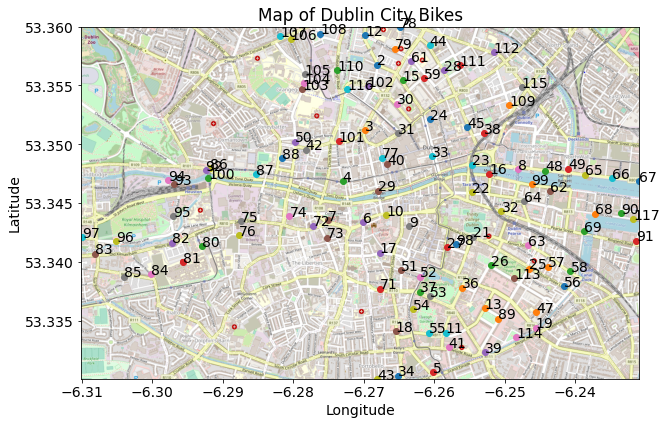
\includegraphics[width=0.7\textwidth]{images/map.png}
\caption{Map of Dublin Bike stations.}
\end{figure}

\begin{figure}[H]
    \centering
    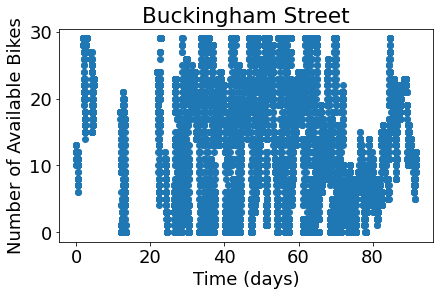
\includegraphics[width=0.5\textwidth]{images/buckingham data.png}
    \caption{Availability of bikes over time at Buckingham Street}
    \end{figure}


\begin{figure}[H]
    \centering
    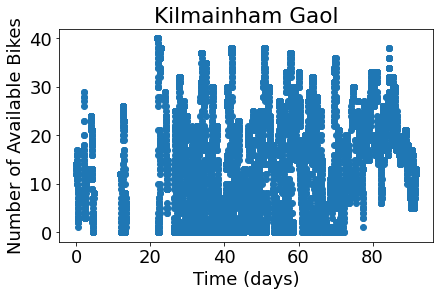
\includegraphics[width=0.5\textwidth]{images/kilmainham data.png}
    \caption{Availability of bikes over time at Kilmainham Gaol}
    \end{figure}
\par 



\subsubsection{Data Cleaning}
As can be seen in figures 2 and 3, much of the data in the first few weeks is missing.
I decided to simply remove the first 27 days in both datasets as 
there was so much missing that it would likely make it more difficult to 
work with the data in a way that didn't negatively affect the performance of the models.
It is likely that there were other missing data points, this is evident in that not every day has the same number of entries (between 287 and 289).
This is unlikey to have any major impact on my predictions as it is very close to 288
(the number of 5 minute time blocks in a day).

\subsubsection{Feature Selection}
The features I took from the datasets are the time and the number of bikes at that time.
This allows other features to be derived from this.
\par 
I turned the time of day into a float (it was slighlty skewed because the first reading of the year was around 6am.)
This was obviously an important feature to take into account as different times of day obviously have different behaviour in terms of bike usage.


\par
The day of week undoubtedly has an effect on how dublin bikes are used. 
This means that it is important to take the day of week into account when training a predictor on this data.
Weekdays can be represented with numbers (e.g. from 1-7) but this could cause problems in linear models.
To counteract this I used one-hot encoding, 
this allows categorical data such as weekday to be presented in such a way that is less likely to cause unnecessary bias.
The downside of this is that it adds many more dimensions to the feature vectors which can make models unnecessarily complex.

\par 
As I was attempting to predict values for the number of bikes available,
I used past values for available bikes.
For each type of prediction I used the 5 previous values for available bikes (for 10 minute ahead prediction I used the values at 10, 15, 20, 25 and 30 minutes earlier. This is the same as what I did for 30 and 60 minute predictions.)

\par 
I also made some new features DB1, DB2, and DDB1DB2 as can be seen in figure 4.
DB1 and DB2 are the differences between number of bikes in the most recent datapoints.
DDB1DB2 is kind of like the 2nd derivative as it is the difference between DB1 and DB2.
I thought that these features would be useful in prediction.

\begin{figure}[H]
    \centering
    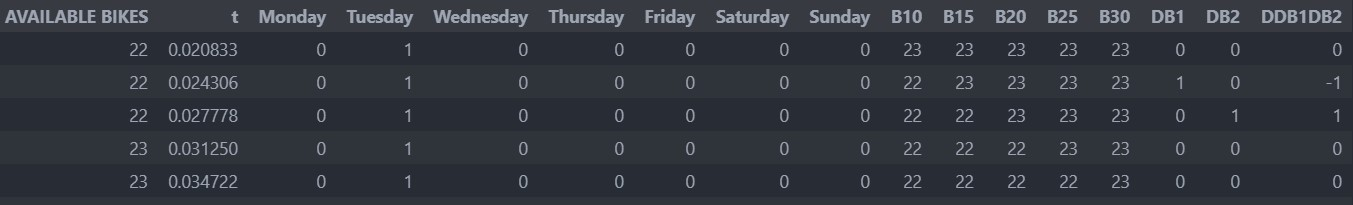
\includegraphics[width=1\textwidth]{images/example_features.jpg}
    \caption{Example of feature dataframe for 10-minute-ahead prediction}
    \end{figure}
\par 

For the ridge regression prediction I also trained similar models with polynomial combinations of the data to see if this better captured the relationships between the different features.
I used every ccombination of features up to a power of 2 which gives 153 features.
This obviously makes a far more complex model and it is far more confusing to figure out what models are doing when there are so many different features.

\par 


\subsection{Ridge Regression}
I initially decided to use ridge regression to predict future values. 
I wanted to use some form of linear regression because I used them for a similar problem in my group project.
Lasso regression is more likely than Ridge to reduce coefficients to zero but I was curious to see how even the lightly weighted parameters were affected so I decided to use ridge regression instead.
\par 

I used 5 fold cross validation to find the ideal value for alpha to use and I found that varying alpha had very little effect until alpha became quite large 
as can be seen in figure 5. 
I decided to use a value of 1 for every model as this value gave a near minimum mean-squared error for every prediction model.
\par 
The metric I used to evaluate performance is mean squared error. 
I feel that this is a suitable metric as it tells us how far off predictions from a model are. 
\par
\begin{figure}[H]
    \centering
    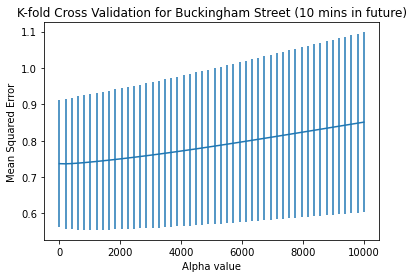
\includegraphics[width=0.5\textwidth]{images/ridge_kfold1.png}
    \caption{K-fold cross validation for ridge regression.}
    \end{figure}
\par 

Training ridge regression on all of the datasets produced very similar graphs so an alpha value of 1 was used for all.

\begin{figure}[H]
    \centering
    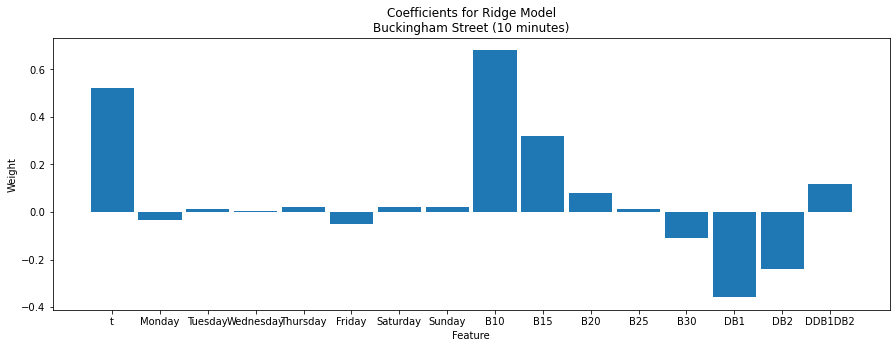
\includegraphics[width=1\textwidth]{images/coefficients1.png}
    \caption{Weighting of coefficients for ridge regressor predicting 10 minutes ahead.}
    \end{figure}
\par 
\begin{figure}[H]
    \centering
    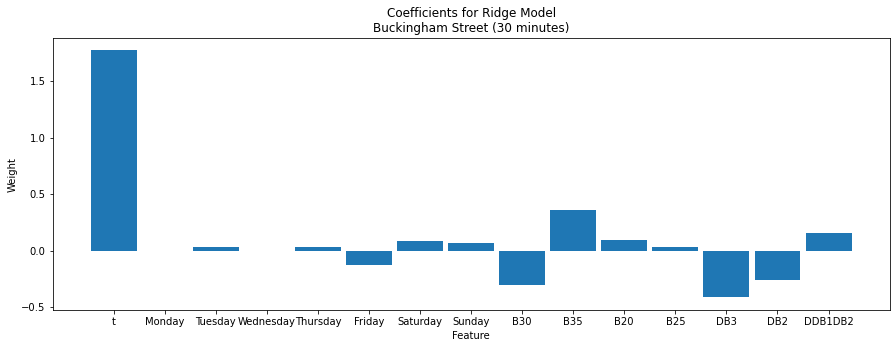
\includegraphics[width=1\textwidth]{images/coefficients3.png}
    \caption{Weighting of coefficients for ridge regressor predicting 30 minutes ahead.}
    \end{figure}
\par 


\begin{figure}[H]
    \centering
    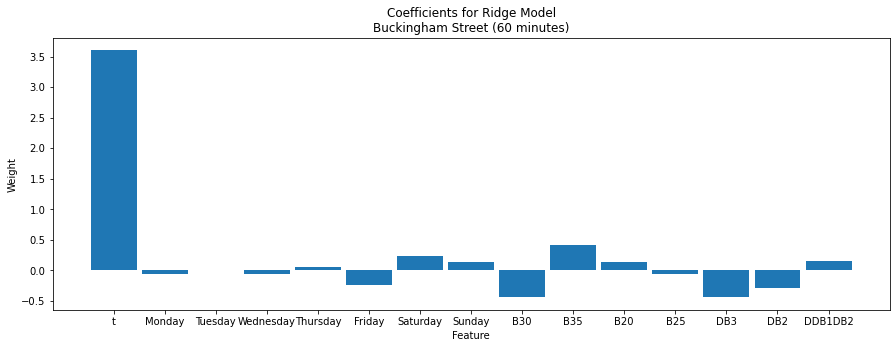
\includegraphics[width=1\textwidth]{images/coefficients5.png}
    \caption{Weighting of coefficients for ridge regressor predicting 60 minutes ahead.}
    \end{figure}
\par 


\subsection{K Neighbours Regression}

I decided to use K-neighbours regression as it works quite differently from ridge regression and is supposedly suitable for predictions in time series data.
I used K-fold cross-validation to tune number of parameters used in training.
Changing the value of p, which affects how distances between pointsare handled, had almost no effect ao I saw no reason to change it from the default.
Changing the leaf size had almost no effect so I saw no reason to change it from the default.
Changing the number of neighbours had a massive effect as can be seen in figure 9.

\begin{figure}[H]
    \centering
    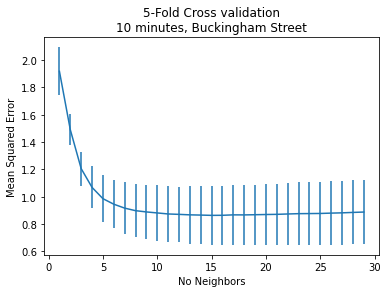
\includegraphics[width=0.5\textwidth]{images/neighbors_kfold1.png}
    \caption{K-fold cross validation for k-neighbors regression.}
    \end{figure}
\par 

All of the cross validation graphs produced similar shapes with the minimum mse being around 10 neighbours and getting diminishing returns for anything higher.

\subsection{Evaluation}
I decided to use what I felt was an appropriate baseline predictor.
The dummy predictor simply predicts that the value will be the same as the previous value.
for example, when predicting 10 minutes ahead the dummy will use the value 10-minutes before.
This makes the dummy predictor quite accurrate and explains why the predictor models did not always outperform it.
\par 
Another reason that the dummy predictor performs comparably to the other predictors is that it chooses integers which the regressors do not do.
This makes the mse quite low as the values often do not change for long periods of time.

\subsubsection{Ridge Regression}
\begin{figure}[H]
    \centering
    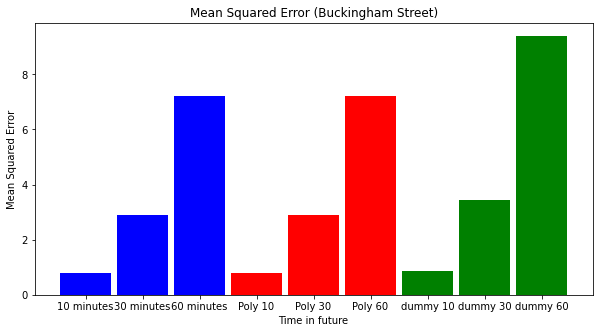
\includegraphics[width=0.6\textwidth]{images/mse1.png}
    \caption{Mean squared error with ridge regression on Buckingham Street.}
    \end{figure}
\par
\begin{figure}[H]
    \centering
    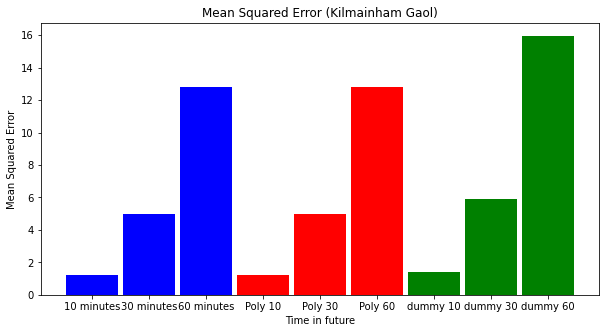
\includegraphics[width=0.6\textwidth]{images/mse2.png}
    \caption{Mean squared error with ridge regression at Kilmainham Gaol.}
    \end{figure}
\par

As can be seen in figures 10 and 11, 
the ridge predictors performed slightly better than the dummy predictors in every scenario.
It is also clear that using the polynomial features had vey little effect on the performance.
As I expectedwould happen, the performance drops as you try to predict further into the future.
This is likely because the features are less related, 
for example the amount of bikes 10 minutes ago is far more related to the current number of bikes than tyhe number of bikes 60 minutes ago.

\begin{figure}[H]
    \centering
    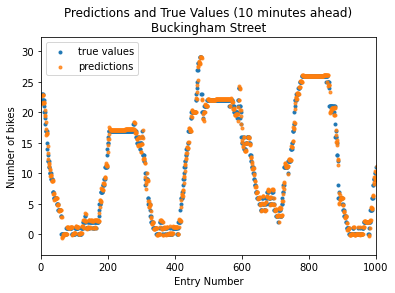
\includegraphics[width=0.5\textwidth]{images/preds1.png}
    \caption{Predictions using ridge regression}
    \end{figure}
\par

As can be seen in figure 12, the predictions look like they are quite accurrate.

\subsubsection{K nearest neighbors Regression}

\begin{figure}[H]
    \centering
    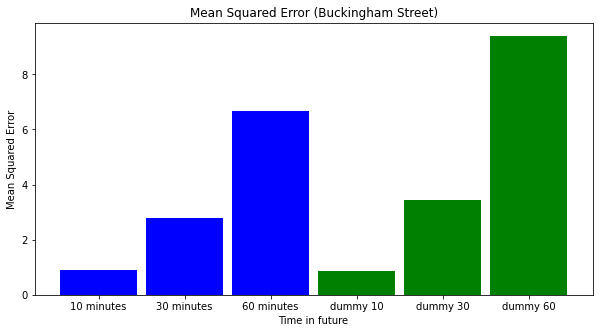
\includegraphics[width=0.6\textwidth]{images/mse3.png}
    \caption{Mean squared error with K-neighbours on Buckingham Street.}
    \end{figure}
\par
\begin{figure}[H]
    \centering
    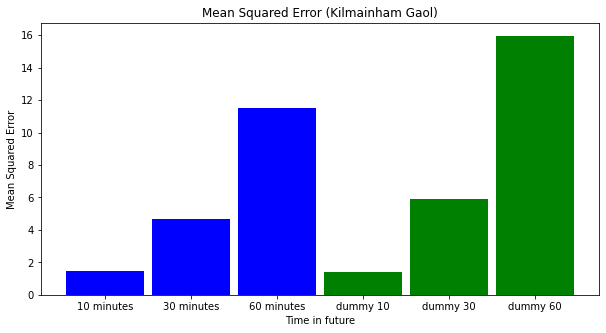
\includegraphics[width=0.6\textwidth]{images/mse4.png}
    \caption{Mean squared error with K nearest neighbors Regression at Kilmainham Gaol.}
    \end{figure}
\par
\begin{figure}[H]
    \centering
    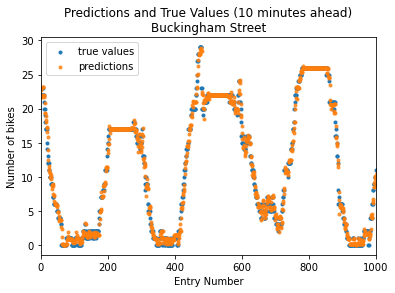
\includegraphics[width=0.5\textwidth]{images/preds7.png}
    \caption{Predictions using K nearest neighbors Regression regression}
    \end{figure}
\par

As can be seen in figures 13 and 14, the K nearest neighbour regressor performs similar to the baseline predictor for short term predictions and performs a bit better for longer term predictions.
The predictions in figure 15 look quite accurrate.


\subsubsection{Comparison}
\begin{figure}[H]
    \centering
    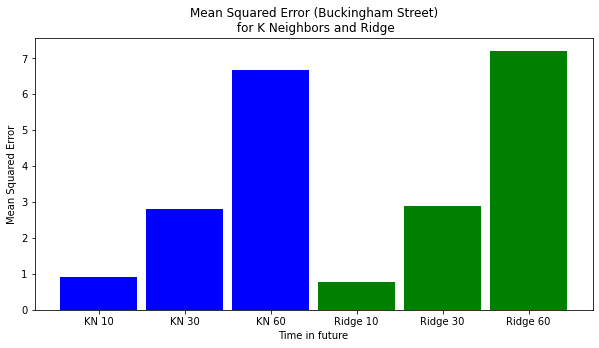
\includegraphics[width=0.6\textwidth]{images/mse5.png}
    \caption{Mean squared error with ridge regression and K nearest neighbors Regression  on Buckingham Street.}
    \end{figure}
\par

\begin{figure}[H]
    \centering
    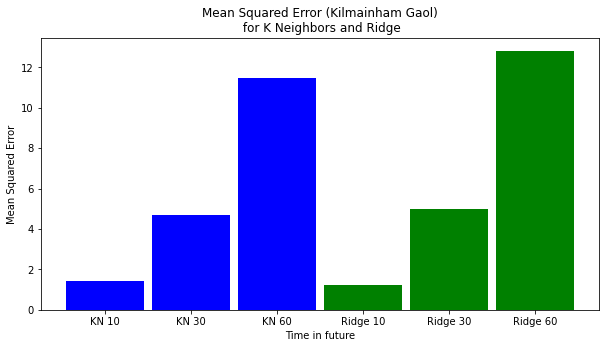
\includegraphics[width=0.6\textwidth]{images/mse6.png}
    \caption{Mean squared error with ridge regression and K nearest neighbors Regression at Kilmainham Gaol.}
    \end{figure}
\par

As can be seen in figures 16 and 17, th Ridge regressor performs slightly better for the short term predictions and the K-nearest neighbors performs slightly better for the longer term predictions.

\par 
Interestingly, the predictions at Kilmainham gaol are worse in every scenario.
Obviously the solutions that work well at Buckingham street are not equally appropriate for every bike station.